% Chapter Template

\chapter{A WEB-BASED PROTOTYPE FOR REMOTE CAR DIAGNOSTICS} % Main chapter title

\label{Chapter4} % Change X to a consecutive number; for referencing this chapter elsewhere, use \ref{ChapterX}

\lhead{Chapter 4. \emph{A WEB-BASED PROTOTYPE FOR REMOTE CAR DIAGNOSTICS}} % Change X to a consecutive number; this is for the header on each page - perhaps a shortened title

%----------------------------------------------------------------------------------------
%	SECTION 1
%----------------------------------------------------------------------------------------
\section{About the application}
This application is a prototype for remote car diagnostics and control, basically is a web app built with a responsive front-end because the target devices are smartphones.
The car is simulated by a car toy made with raspberry pi (Figure \ref{fig:Raspberry}) and a car chassis development kit (Figure \ref{fig:car_chassis}). 

\subsubsection{Dashboard}
In to the dashboard (Figure \ref{fig:dashboard}) we can see principal levels and temperatures from the car, all dates are storage into a NoSQL database, so you can see some history of the oil level for example, the dates are dummy data for now just some random numbers.
\newpage
\begin{figure}[h!]
  \centering
    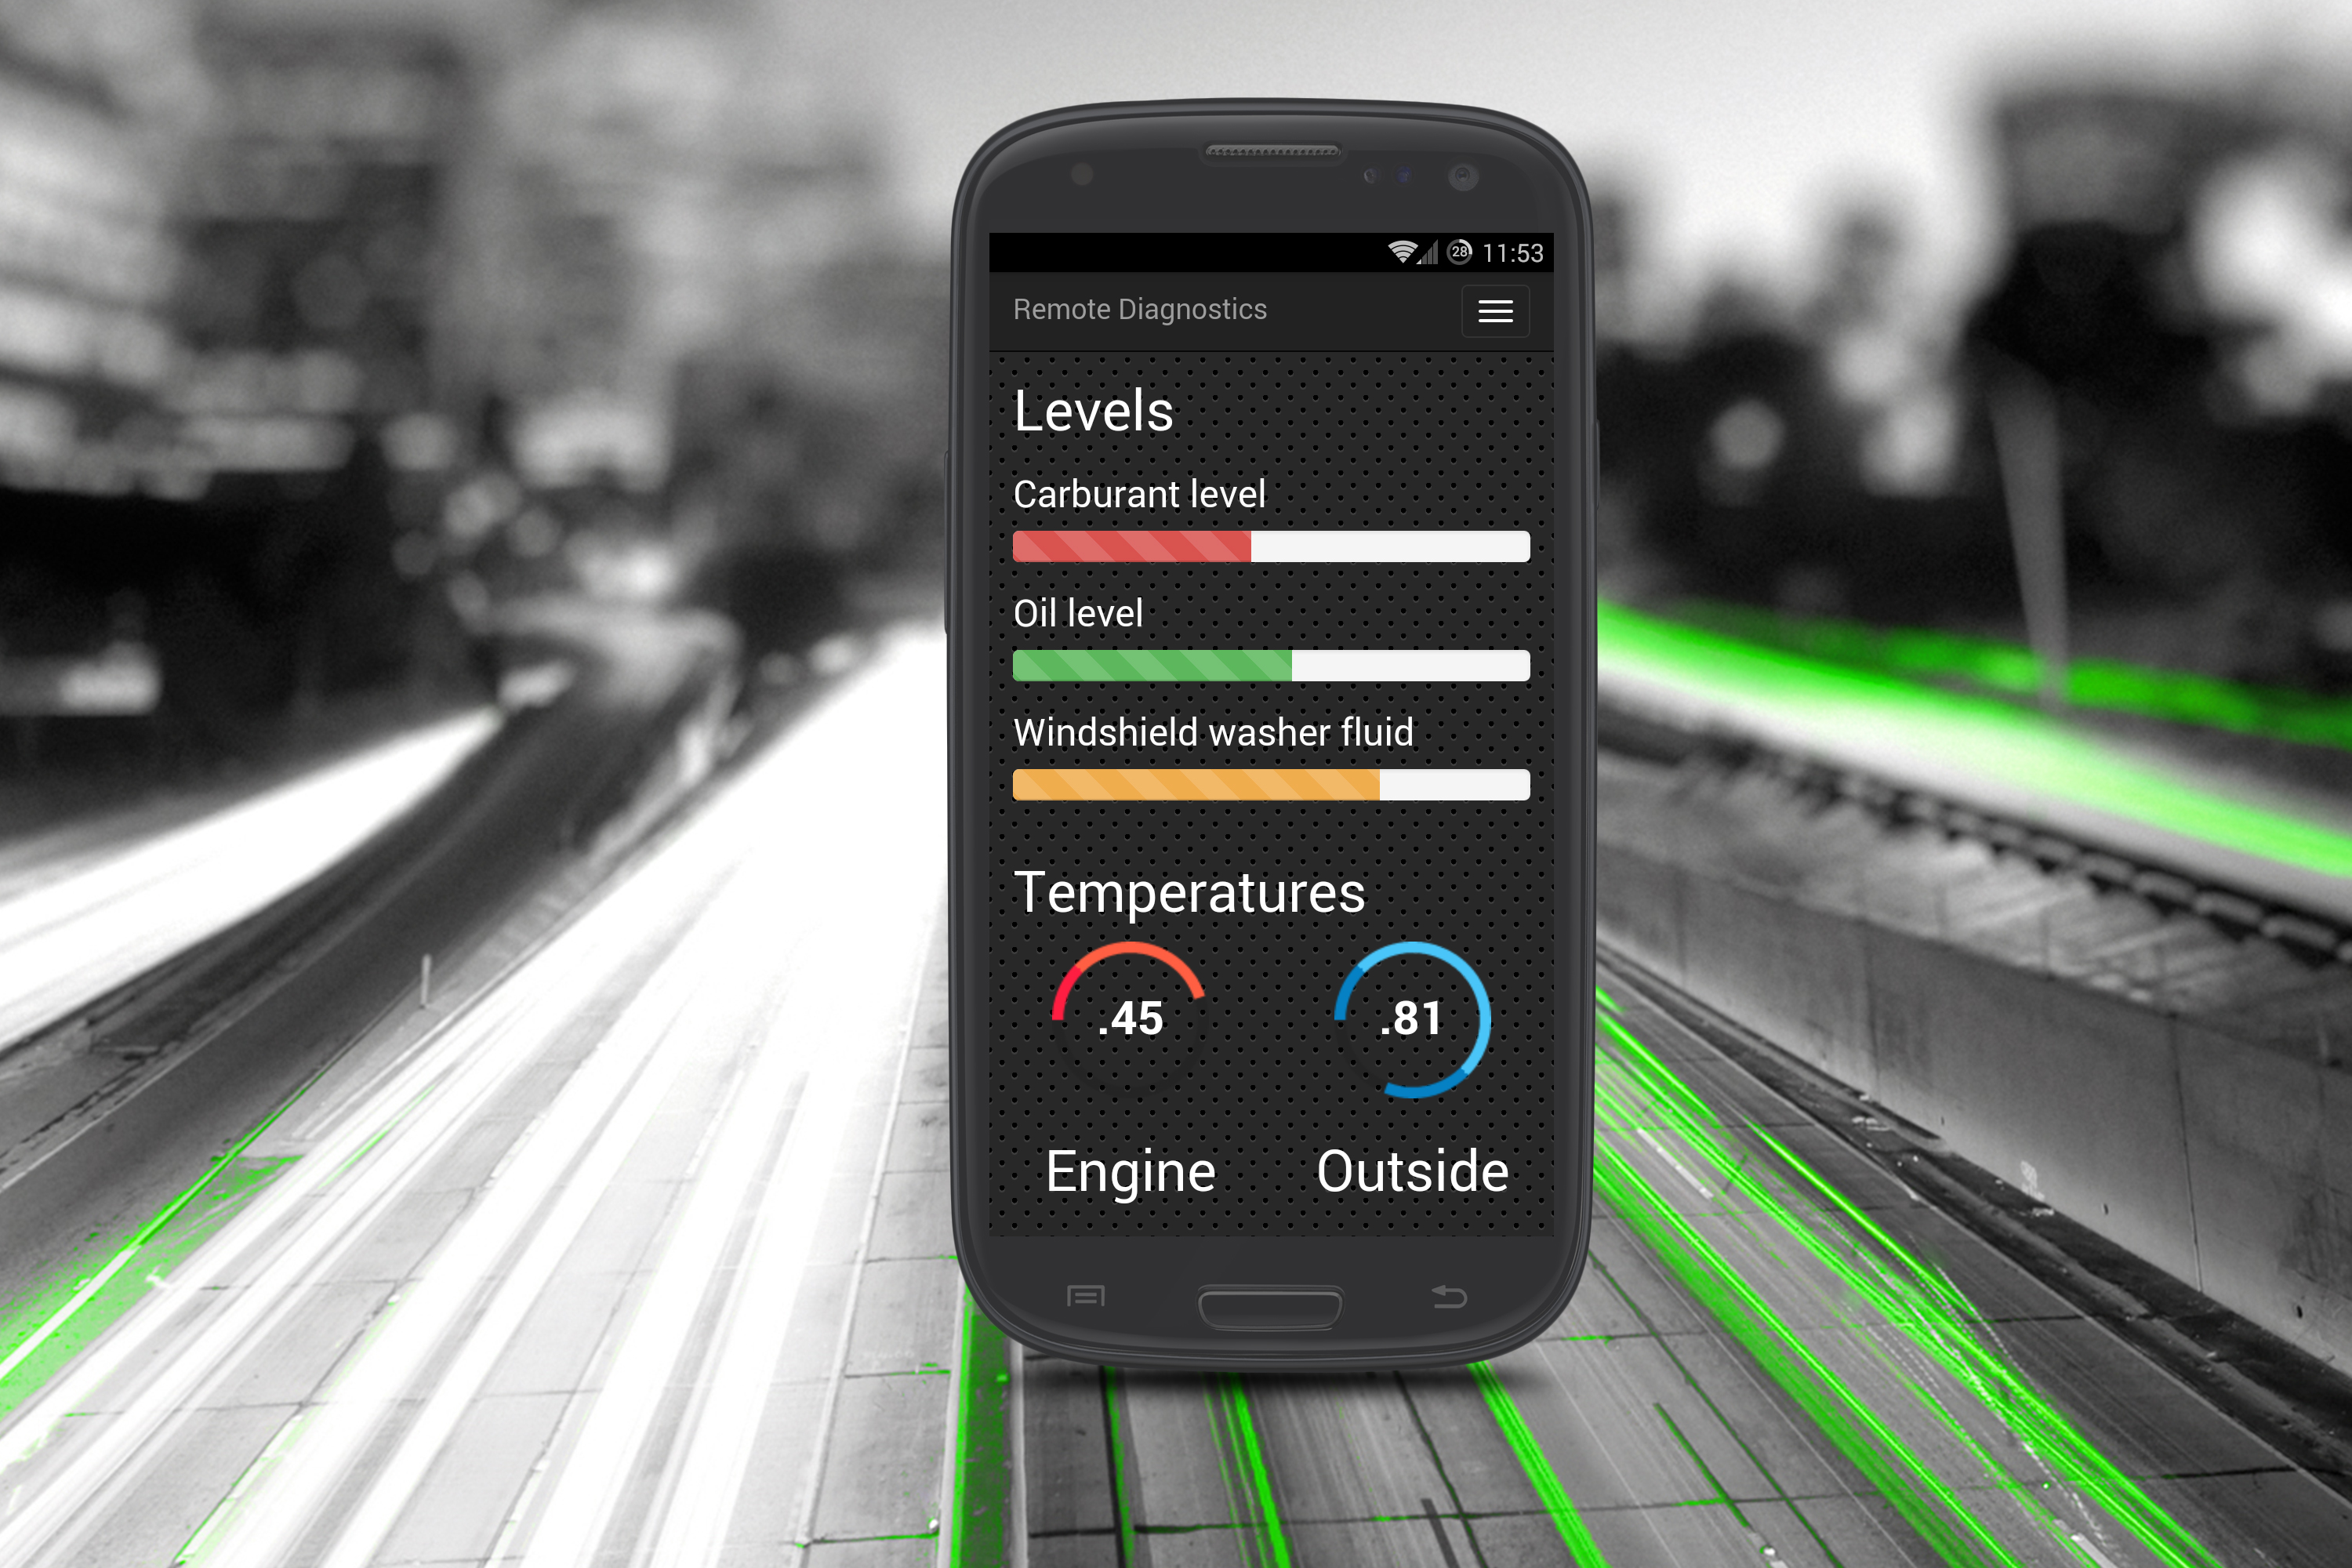
\includegraphics[width=1\textwidth]{./Pictures/dashboard.jpg}
  \rule{1\textwidth}{1pt}
 \caption{Dashboard}
  \label{fig:dashboard}
\end{figure}
%-----------------------------------
%	SUBSECTION 1
%-----------------------------------
\subsection{Controllers}
For the remote control of the car i made three kind of controller:
\begin{itemize}
  \item Keyboard Controller (Figure \ref{fig:keyboard_controller})
  \item Gyroscope Controller (Figure \ref{fig:gyroscope_controller}) 
  \item Speech Controller (Figure \ref{fig:speech_controller})
\end{itemize}
\subsubsection{Keyboard Controller}
The keyboard controller (Figure \ref{fig:keyboard_controller}) is pretty simple, just press the direction where you want to direct the car.
\begin{figure}[h!]
  \centering
    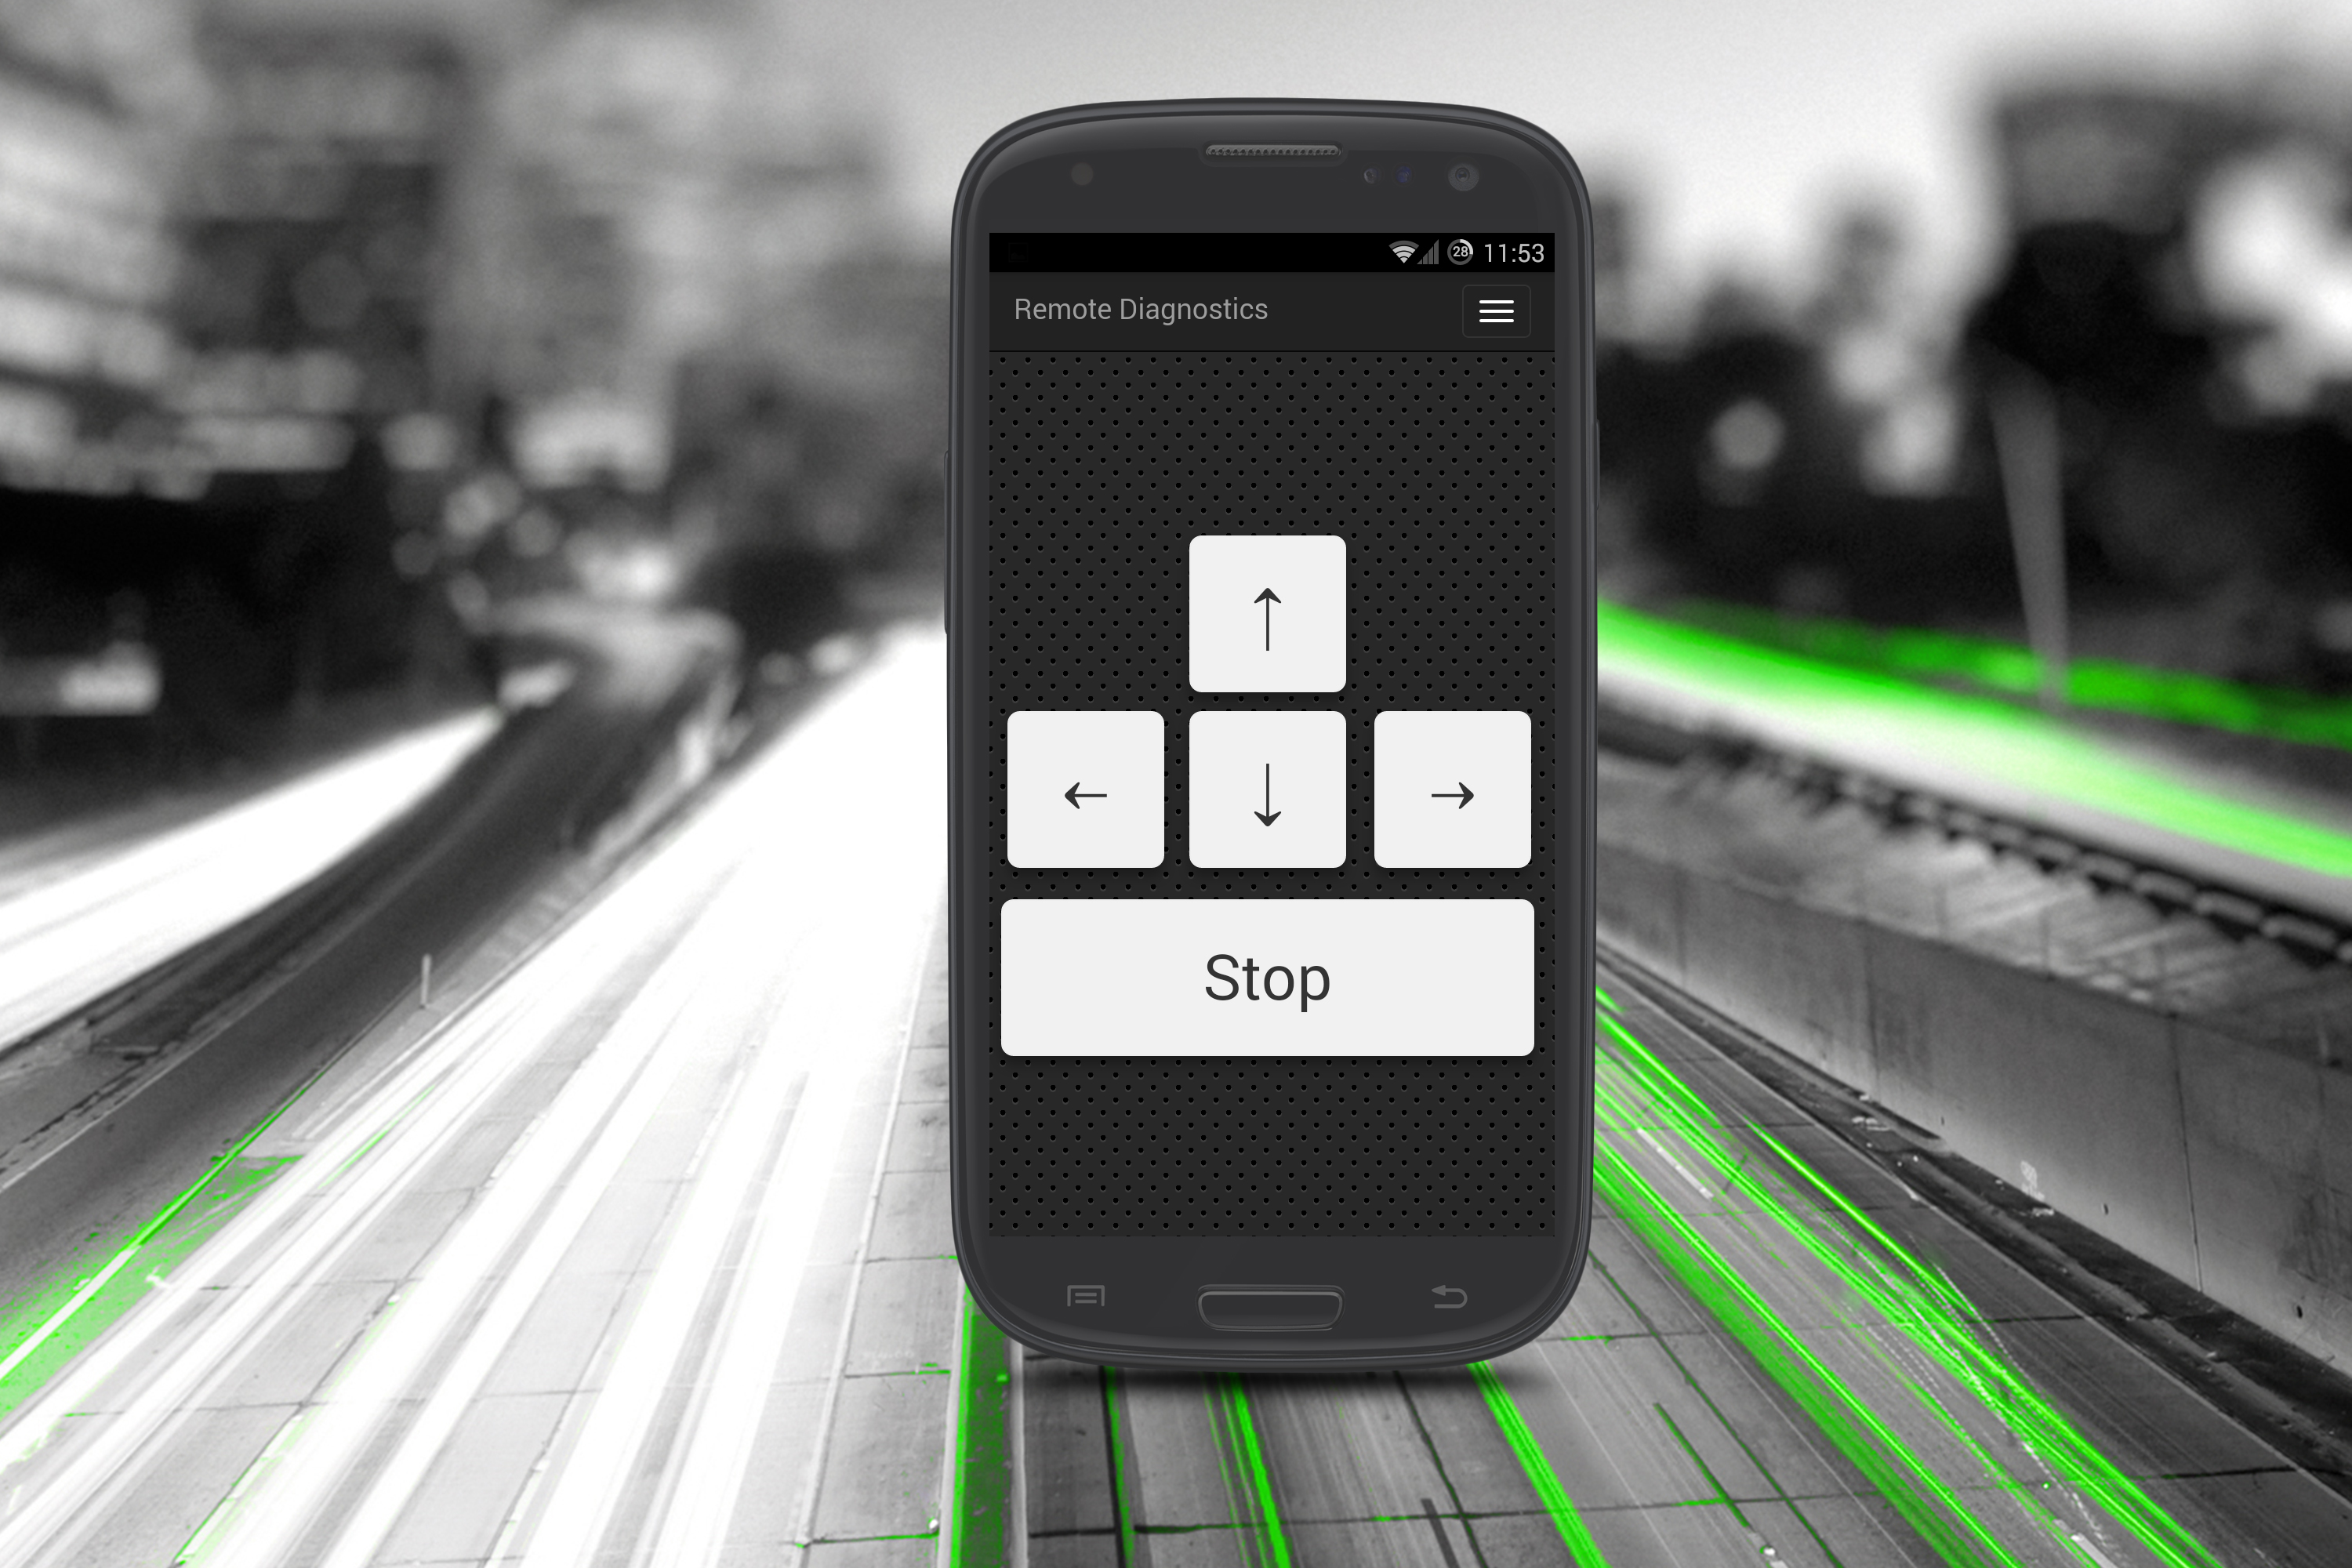
\includegraphics[width=1\textwidth]{./Pictures/keyboard_controller.jpg}
  \rule{1\textwidth}{1pt}
 \caption{Keyboard Controller}
 \label{fig:keyboard_controller}
\end{figure}
\subsubsection{Gyroscope Controller}
For control the car with the gyroscope controller(Figure \ref{fig:gyroscope_controller}) grab the phone with the display facing upwards and incline front,back,left and right to stop just keep the phone horizontally. 
\begin{figure}[h!]
  \centering
    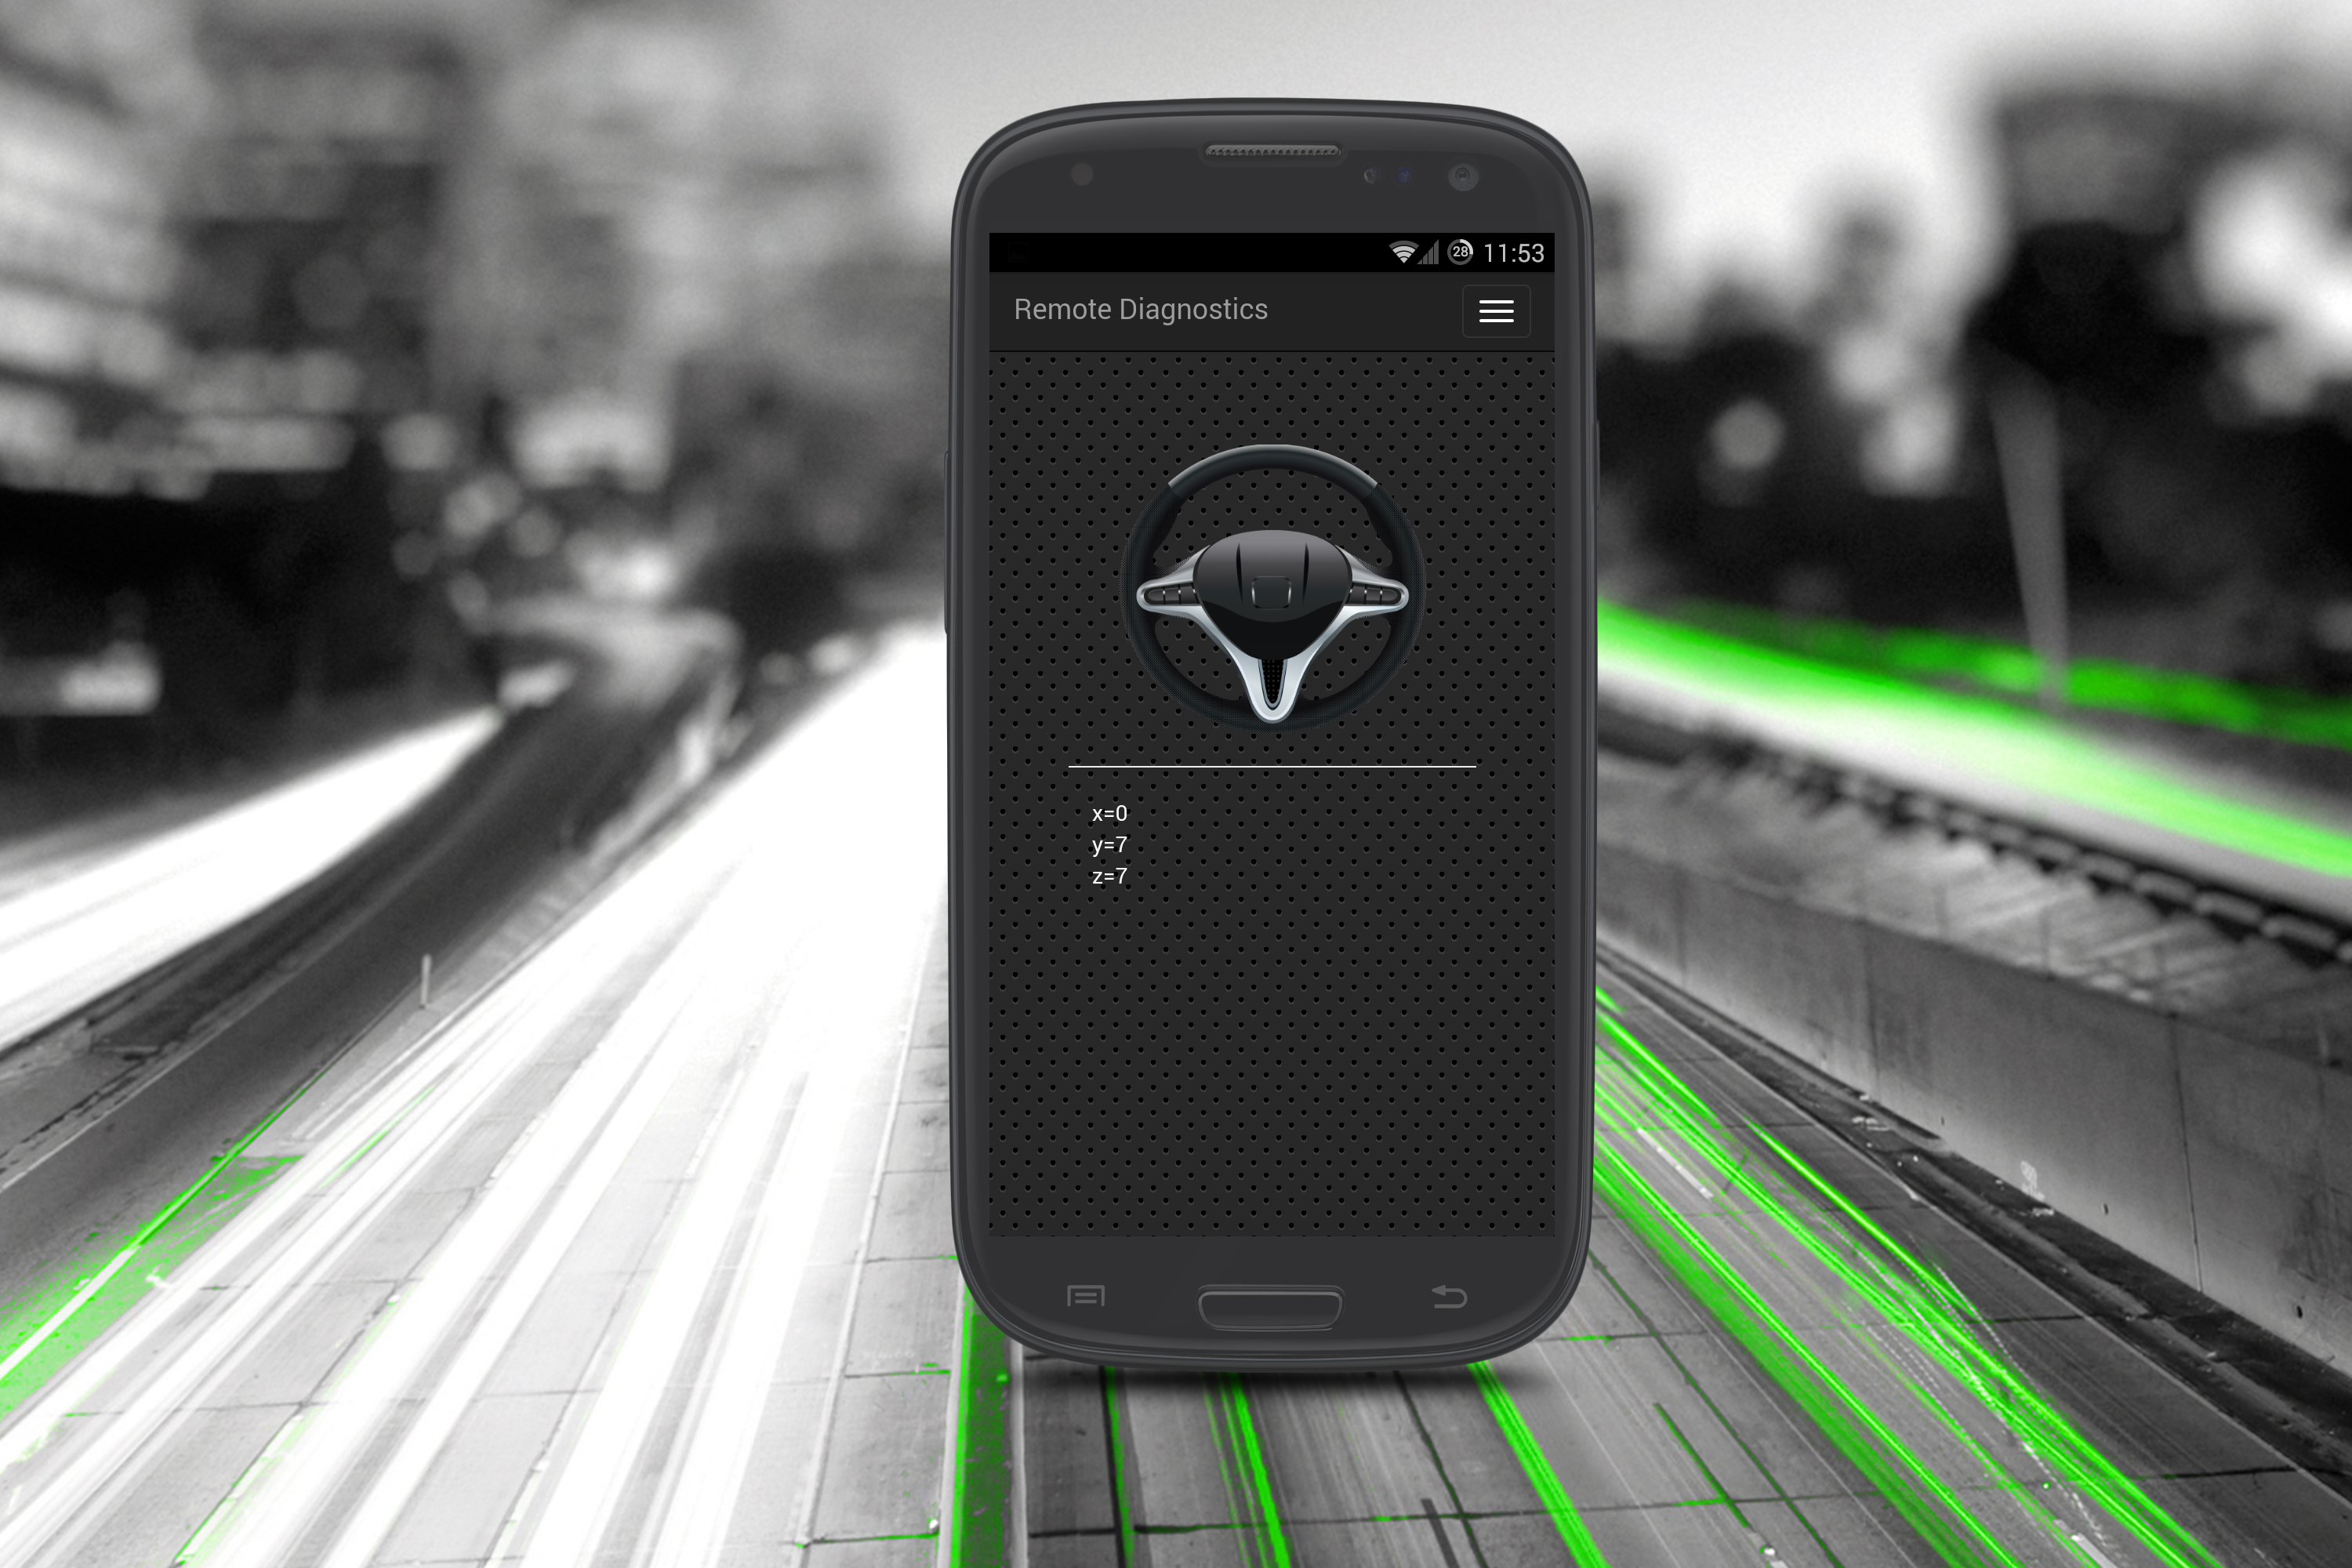
\includegraphics[width=1\textwidth]{./Pictures/gyroscope_controller.jpg}
  \rule{1\textwidth}{1pt}
 \caption{Gyroscope Controller}
  \label{fig:gyroscope_controller}
\end{figure}

\subsubsection{Speech Controller}
With this controller just ``talk''  with the phone some simple commands like ``left'',``right'',``up'',``down'' and ``stop''.(Figure \ref{fig:speech_controller})

\begin{figure}[h!]
  \centering
    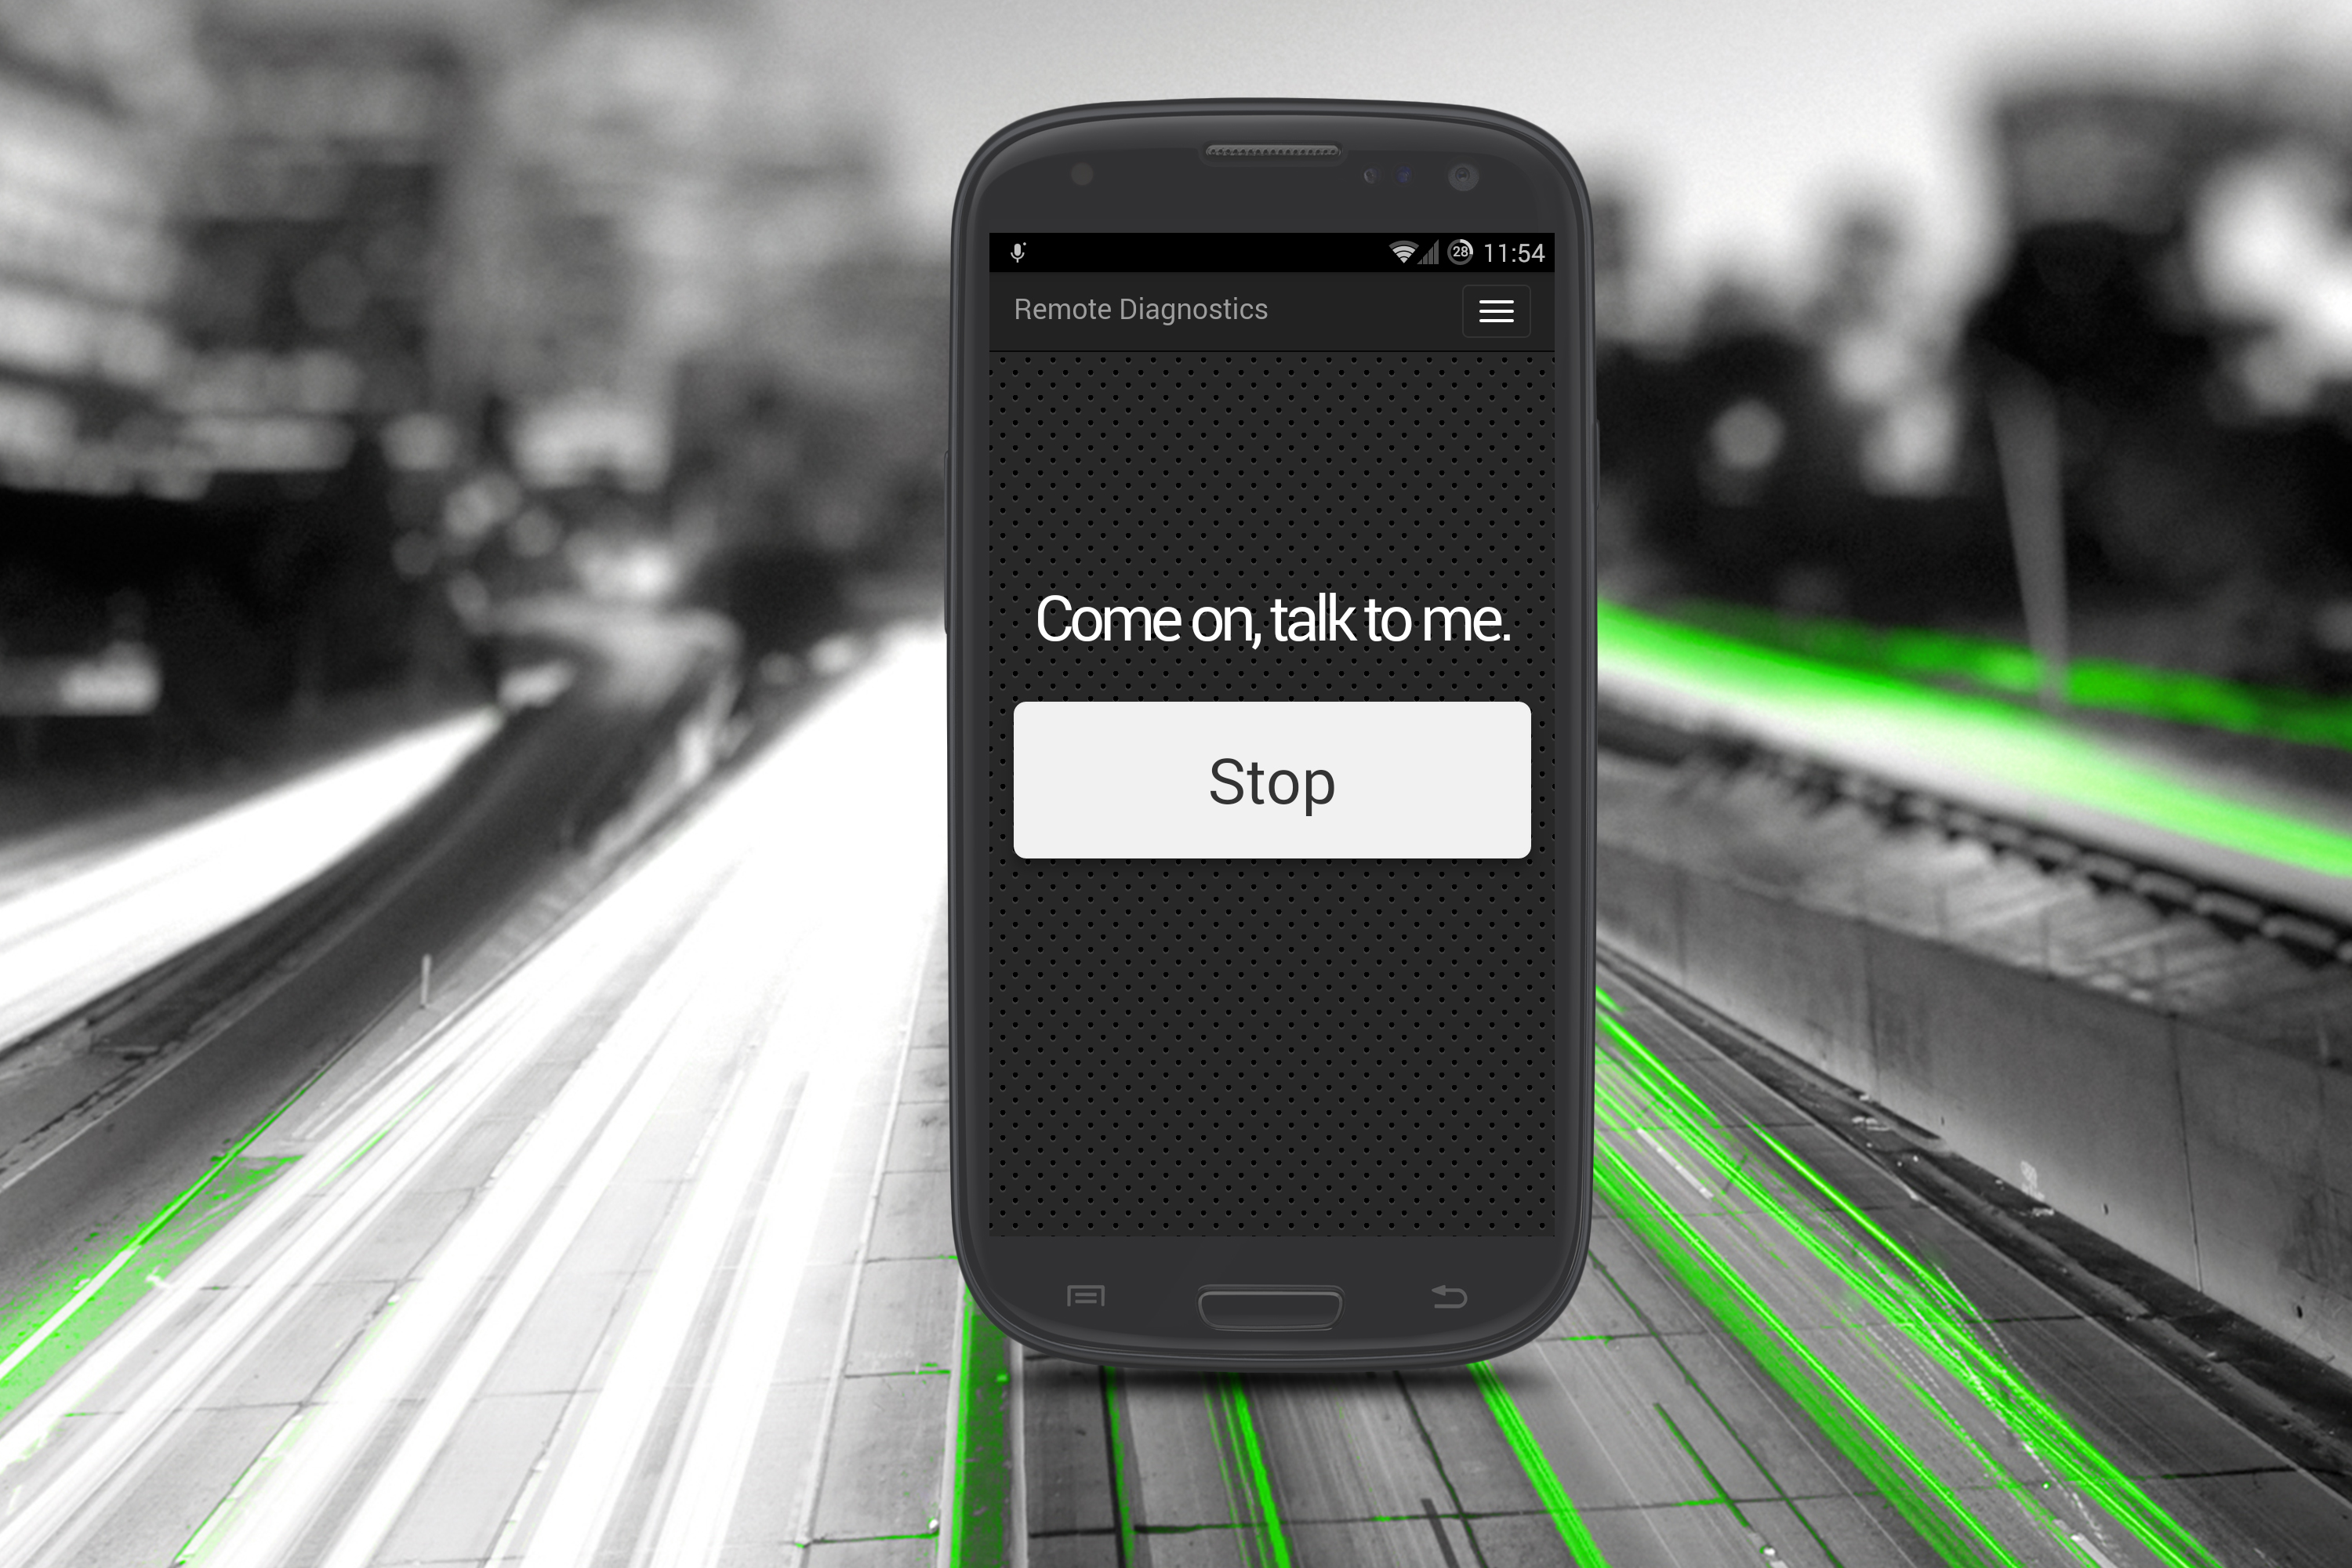
\includegraphics[width=1\textwidth]{./Pictures/speech_controller.jpg}
  \rule{1\textwidth}{1pt}
 \caption{Speech Controller}
  \label{fig:speech_controller}
\end{figure}


\hfill \break
%-----------------------------------
%	SUBSECTION 2
%-----------------------------------
\section{Why? and How?}
\paragraph*{Why nodejs?}
I choose node js because i like JavaScript and this is the most popular language at this moment for web development, and with node js you can write javascript for the back-end of the app not just for front-end in conclusion: JavaScript everywhere!
